\Problem{Японский кроссворд}{1}{64}{inputX.txt}{outputX.txt}

В этой задаче вам предстоит написать программу, решающую упрощенный японский кроссворд.

Упрощенный японский кроссворд~--- это головоломка, в которой надо построить такое поле
(каждая клетка либо белая, либо черная), которое соответствует заданной информации для строк и столбцов.
Для каждой строки и каждого столбца задано количество блоков из черных клеток.
Ваша задача~--- построить такое поле, для которого все эти количества имеют место быть.

Например, если размеры поля $n = 3$, $m = 5$, а количества блоков для строк это $[2, 3, 2]$, а для столбцов~--- $[1, 0, 1, 2, 1]$, то решение может выглядеть так:

\begin{center}
	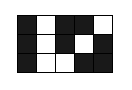
\includegraphics[width=200pt,natwidth=680,natheight=544]{tasks/crossword/statements/images/crossword.png}
\end{center}

Гарантируется, что для каждого теста, на котором будет запущена ваша программа, хотя бы одно решение головоломки существует.

\Input
В первой строке входных данных записаны два целых числа $n$, $m$~--- количество строк и столбцов соответственно.

Вторая строка содержит nnn целых чисел $a_1, a_2, ..., a_n$​, где $a_i$​~--- количество черных блоков в $i$-й строке искомого поля.

Аналогично, третья строка содержит mmm целых чисел $b_1, b_2, ..., b_m$​, где $b_i$​~--- количество черных блоков в $i$-м столбце искомого поля.

Гарантируется, что хотя бы одно решение головоломки существует.

\Output
Выведите любое из возможных решений. Ваш вывод должен содержать $n$ строк по $m$ символов в каждой из них.
Белую ячейку следует обозначать символом «\texttt{.}», а черную~--- символом «\texttt{#}».

\Samples
\BeginTests
	\Test{tasks/crossword/tests/samples}{01}{01.a}
	\Test{tasks/crossword/tests/samples}{02}{02.a}
	\Test{tasks/crossword/tests/samples}{03}{03.a}
\EndTests

\Scoring
Вы получите $10$ баллов, если смогли решить задачу. Если же не удалось получить решение, то вы получите: $10 \cdot \frac{1 + Ans}{1 + Out}$, где $Ans$~---
результат авторов, где сумма квадратов разниц между $a_i$ и полученным количеством блоков и сумма квадратов разниц между $b_i$ и полученным количество блоков,
а $Out$~--- ответ участника.

\EndProblem
